\documentclass[a4paper,10pt]{article}
\usepackage[lmargin=2.0cm, rmargin=1.0cm,tmargin=3.5cm,bmargin=1.5cm]{geometry}
\usepackage{color,graphics}
\usepackage[export]{adjustbox}
\usepackage{lipsum}
\usepackage{comment}
\usepackage{graphicx}

\usepackage{listings}
\usepackage[scaled=0.75]{helvet}

\begin{document}
\setcounter{secnumdepth}{-1} 

\begin{center}
\textbf{\LARGE Running Hadoop On Ubuntu Linux (Single-Node Cluster)}
\end{center}

\raggedright Expt No: 2 \hfill \raggedleft March  07, 2019 \\ 

\raggedright Author: Subalakshmi Shanthosi S  (186001008) \par 

\noindent\makebox[\linewidth]{\rule{\textwidth}{1pt}} 

\section{Aim}
To configure and install  Hadoop  in Ubuntu 16.04 LTS OS flavour.

\section{Software's Used}
\begin{itemize}
  \item Ubuntu  16.04 LTS
  \item Hadoop 2.7.3
\end{itemize}

\section{Description}
Installation of Oracle VirtualBox with guest Operating System as Ubuntu 16.04.Installation of neccessary packages namely - openssh-server,openssh-client,java,hadoop in the created virtualbox instance.
\section{Procedure}

\begin{enumerate}
	\item Launch Ubuntu 16.04 LTS.
	\item Login to the OS with sudo permission and install the following packages using apt-get command
	\begin{itemize}
		\item openssh-server
		\item openssh-client
		\item java jdk 8
		\item javac compiler
                     \item hadoop 2.7.3
	\end{itemize}
\pagebreak
\end{enumerate}

\section{Output}
\begin{figure}[h]
	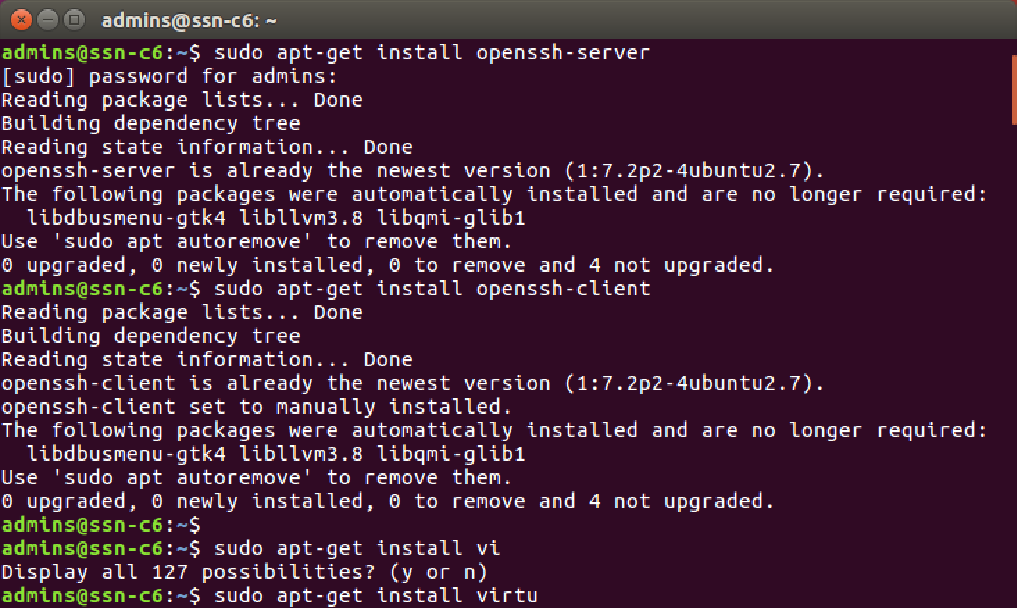
\includegraphics[scale=0.30,center]{exptTwoScreenShot/fig1.png}
	\caption{Install openssh-server,openssh-client in Ubuntu OS.}
	\label{fig:1}
	
\end{figure}
\begin{figure}[h]
	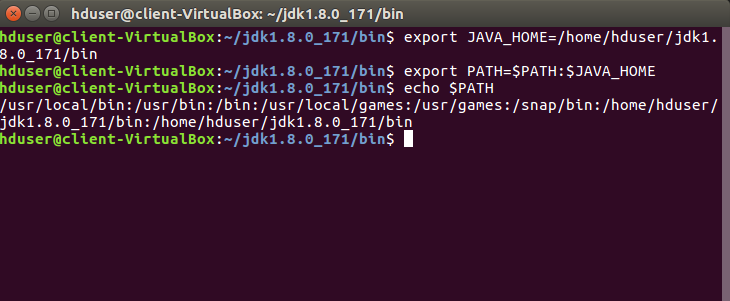
\includegraphics[scale=0.34,center]{exptTwoScreenShot/fig2.png}
	\caption{Setting Java Home environment variable to the specified download path of JDK-1.7.}
	\label{fig:2}
\end{figure}

\begin{figure}[h]
	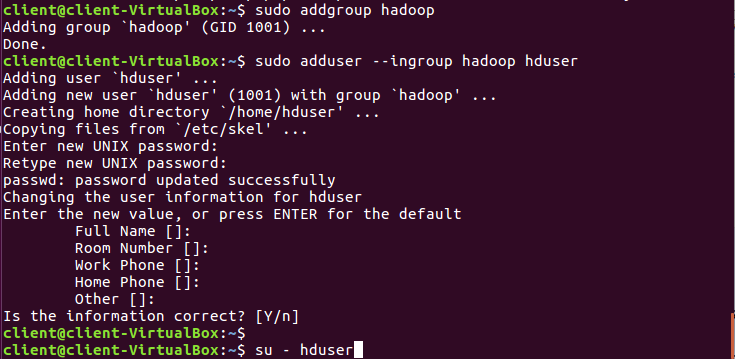
\includegraphics[scale=0.34,center]{exptTwoScreenShot/fig3.png}
	\caption{Adding a dedicated hadoop system user.}
	\label{fig:3}
\end{figure}
\newpage
\begin{figure}[h]
	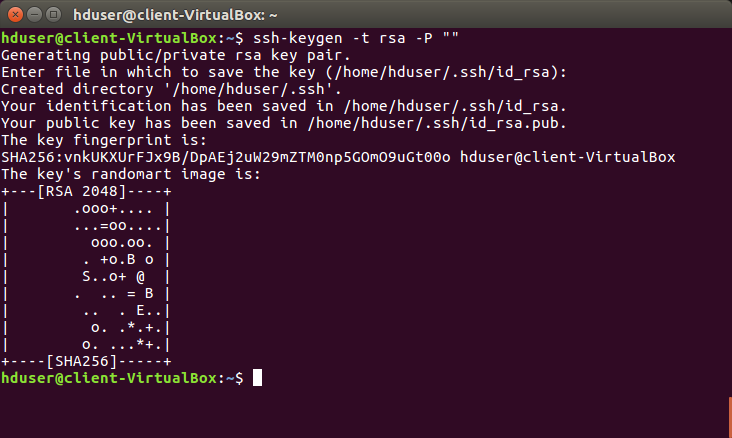
\includegraphics[scale=0.30,center]{exptTwoScreenShot/fig4.png}
	\caption{Configuring SSH in newly created user.}
	\label{fig:4}
\end{figure}

\begin{figure}[h]
	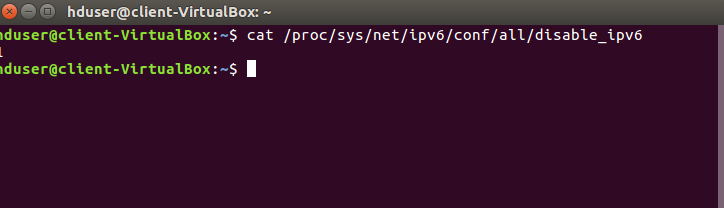
\includegraphics[scale=0.34,center]{exptTwoScreenShot/fig5.png}
	\caption{Disabling IPv6 in the newly created user account.}
	\label{fig:5.1}
\end{figure}

\begin{figure}[h]
	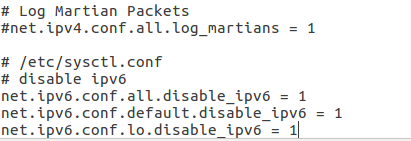
\includegraphics[scale=0.34,center]{exptTwoScreenShot/fig5Two.png}
	\caption{Disabling IPv6 in the newly created user account.}
	\label{fig:5.2}
\end{figure}

\begin{figure}[h]
	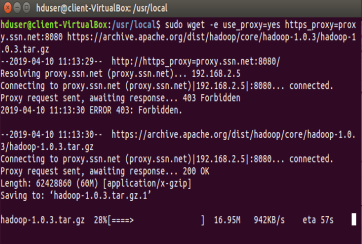
\includegraphics[scale=0.30,center]{exptTwoScreenShot/fig6.png}
	\caption{Installation of Hadoop 2.7.3 in new user login.}
	\label{fig:6}
\end{figure}
\newpage
\begin{figure}[h]
	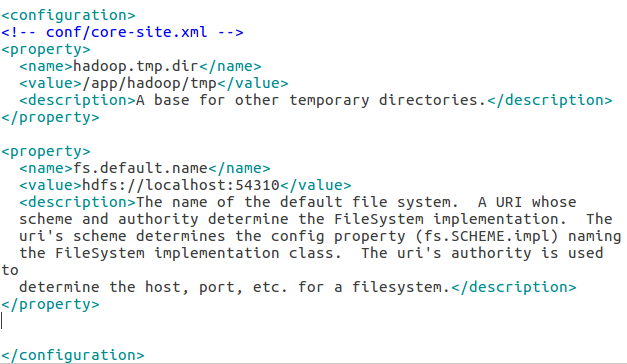
\includegraphics[scale=0.30,center]{exptTwoScreenShot/fig7.png}
	\caption{Configuring hadoop core-site.xml .}
	\label{fig:7}
\end{figure}

	\begin{figure}[h]
		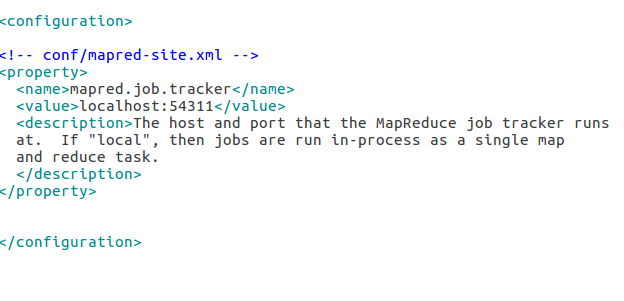
\includegraphics[scale=0.30,center]{exptTwoScreenShot/fig8.png}
		\caption{Configuring Hadoop MapReduce.}
		\label{fig:8}
	\end{figure}
	
	\begin{figure}[h]
		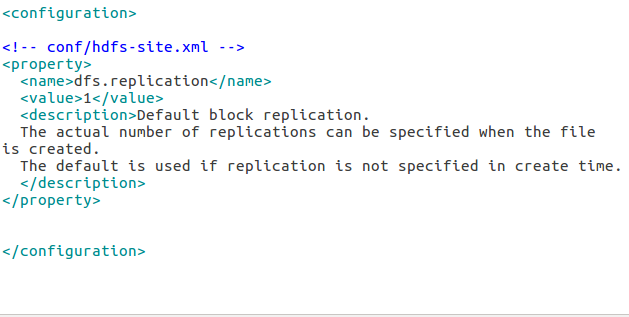
\includegraphics[scale=0.30,center]{exptTwoScreenShot/fig9.png}
		\caption{Configuring Hadoop HDFS Site.}
		\label{fig:9}
	\end{figure}

\pagebreak

	\begin{figure}[h]
		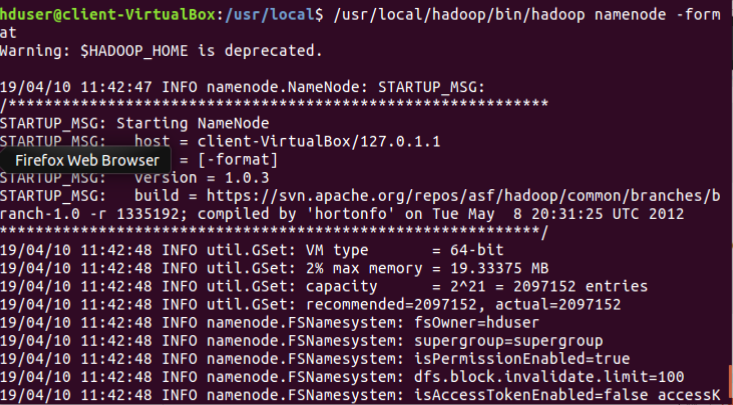
\includegraphics[scale=0.30,center]{exptTwoScreenShot/fig10.png}
		\caption{Formatting HDFS file system via the NameNode.}
		\label{fig:8}
	\end{figure}


\section{Result}
Thus the oracle virtualbox VM instance is sucessfully created with Ubuntu 16.04 OS version and required packages are installed.

\end{document}
